% !TeX root = ../main.tex
% Add the above to each chapter to make compiling the PDF easier in some editors.

\chapter{Experimental Results and Analysis}\label{chapter:presentation_of_the_results}

\section{Evaluation Metrics}

To appreciate the quality of the estimations, the most widely used pose error functions are the \ac{ADD} and the \ac{ADD-S} metrics, both introduced by Hinterstoisser et al. \cite{10.1007/978-3-642-37331-2_42}. For an object model $\mathcal{M}$, we compute the average distance to the corresponding model point. Therefore the error of an estimated pose $\hat{\bm{\mathrm{P}}}=(\hat{\bm{\mathrm{R}}},\,\hat{\bm{\mathrm{t}}})$ w.r.t. the ground truth pose $\bar{\bm{\mathrm{P}}}=(\bar{\bm{\mathrm{R}}},\,\bar{\bm{\mathrm{t}}})$ is calculated as follows:

\begin{align}
	\textit{\footnotemark}e_\mathrm{ADD}(\hat{\bm{\mathrm{P}}},\,\bar{\bm{\mathrm{P}}},\,\mathcal{M})&\stackrel{\text{def.}}{=}\underset{\bm{\mathrm{x}}\in\mathcal{M}}{\mathrm{avg}}\norm\bigg{\bar{\bm{\mathrm{P}}}\bm{\mathrm{x}}^\star-\hat{\bm{\mathrm{P}}}\bm{\mathrm{x}}^\star}_2 \\
	&=\underset{\bm{\mathrm{x}}\in\mathcal{M}}{\mathrm{avg}}\norm\bigg{(\bar{\bm{\mathrm{R}}}\bm{\mathrm{x}}+\bar{\bm{\mathrm{t}}})-(\hat{\bm{\mathrm{R}}}\bm{\mathrm{x}}+\hat{\bm{\mathrm{t}}})}_2
\end{align}
\footnotetext{In this context, the vector $\bm{\mathrm{x}}^\star$ represents a vector that has been extended by appending a 1, specifically for the purpose of matrix multiplication.}

\noindent When the model $\mathcal{M}$ has symmetries that leads to indistinguishable views, the error is computed as the average distance to the closest model point:
 
\begin{align}
	e_{\mathrm{ADD}\text{-}\mathrm{S}}(\hat{\bm{\mathrm{P}}},\,\bar{\bm{\mathrm{P}}},\,\mathcal{M})&\stackrel{\text{def.}}{=} \underset{\bm{\mathrm{x}}_1\in\mathcal{M}}{\mathrm{avg}}\min\limits_{\bm{\mathrm{x}}_2\in\mathcal{M}}\norm\bigg{\bar{\bm{\mathrm{P}}}\bm{\mathrm{x}}_1^\star-\hat{\bm{\mathrm{P}}}\bm{\mathrm{x}}_2^\star}_2 \\
	&=\underset{\bm{\mathrm{x}}_1\in\mathcal{M}}{\mathrm{avg}}\min\limits_{\bm{\mathrm{x}}_2\in\mathcal{M}}\norm\bigg{(\bar{\bm{\mathrm{R}}}\bm{\mathrm{x}}_1+\bar{\bm{\mathrm{t}}})-(\hat{\bm{\mathrm{R}}}\bm{\mathrm{x}}_2+\hat{\bm{\mathrm{t}}})}_2
\end{align}

\bigskip

It's important to point out that $e_{\mathrm{ADD}\text{-}\mathrm{S}}$ is more lenient compared to $e_\mathrm{ADD}$, and should only be applied in cases where there is a definite presence of symmetry in the object and the estimated pose is already notably precise. Otherwise, using $e_{\mathrm{ADD}\text{-}\mathrm{S}}$ becomes irrelevant since the estimation would be unfairly advantaged. In the illustrations below, we consistently provide both metrics, however it is up to the reader to assess the relevance of $e_{\mathrm{ADD}\text{-}\mathrm{S}}$ based on the observed spacecraft. 


\section{Vizualisation and Quantitative Evaluation}
\fancyhead[C]{\small\textsc{4.2. Vizualisation and Quantitative Evaluation}}

With all these tools and the modifications made, we are now in a position to test Gen6D as-is, that is without retraining the model. For each spacecraft, we select approximately $200$ reference images from a random image folder, and about ten hand-picked query images to ensure the best possible conditions. Indeed, we aim for the object to be in the foreground, fully within the frame, and under good lighting conditions. Since we are on the \ac{ESA} competition track with 3D target models included, we skip the \ac{SFM} step with Colmap. Below are the best pose estimations made by Gen6D for each of the four objects.
 
\bigskip
\bigskip
\bigskip
\bigskip
 
\begin{figure}[h]
    \centering
    \begin{minipage}{0.45\linewidth}
        \centering
        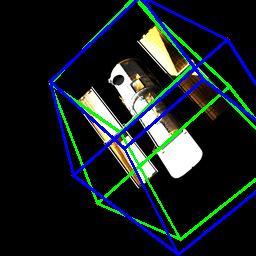
\includegraphics[width=\linewidth]{data/fig3.jpg} % First image
        \caption{Hubble Space Telescope, no background, 256x256 query image, $e_\mathrm{ADD}=2.925$, $e_{\mathrm{ADD}\text{-}\mathrm{S}}=1.183$ }
        \label{fig:fig3}
    \end{minipage}\hfill
    \begin{minipage}{0.45\linewidth}
        \centering
        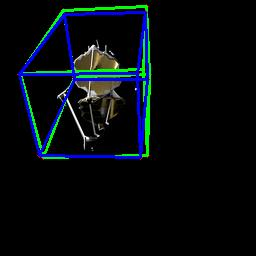
\includegraphics[width=\linewidth]{data/fig4.jpg} % Second image
        \caption{James Webb ST, no background, 256x256 query image, $e_\mathrm{ADD}=1.415$, $e_{\mathrm{ADD}\text{-}\mathrm{S}}=0.808$ }
        \label{fig:fig4}
    \end{minipage}
\end{figure}

\bigskip
\bigskip

\begin{figure}[h]
    \centering
    \begin{minipage}{0.45\linewidth}
        \centering
        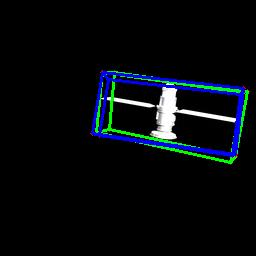
\includegraphics[width=\linewidth]{data/fig5.jpg} % First image
        \caption{Cosmos Link, no background, 256x256 query image, $e_\mathrm{ADD}=1.718$, $e_{\mathrm{ADD}\text{-}\mathrm{S}}=0.383$ }
        \label{fig:fig5}
    \end{minipage}\hfill
    \begin{minipage}{0.45\linewidth}
        \centering
        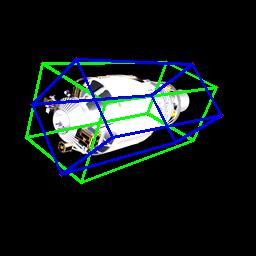
\includegraphics[width=\linewidth]{data/fig6.jpg} % Second image
        \caption{Rocket Body, no background, 256x256 query image, $e_\mathrm{ADD}=1.713$, $e_{\mathrm{ADD}\text{-}\mathrm{S}}=0.252$ }
        \label{fig:fig6}
    \end{minipage}
\end{figure}

\newpage

\begin{figure}[h]
    \centering
    \begin{minipage}{0.45\linewidth}
        \centering
        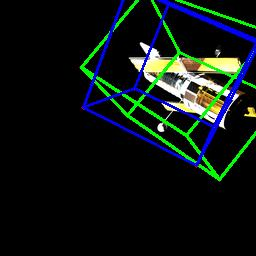
\includegraphics[width=\linewidth]{data/fig7.jpg} % First image
        \caption{Hubble Space Telescope, no background, 256x256 query image, $e_\mathrm{ADD}=6.514$, $e_{\mathrm{ADD}\text{-}\mathrm{S}}=1.571$ }
        \label{fig:fig7}
    \end{minipage}\hfill
    \begin{minipage}{0.45\linewidth}
        \centering
        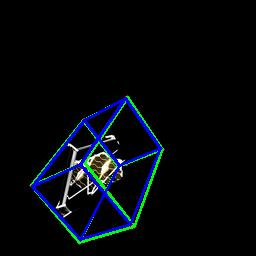
\includegraphics[width=\linewidth]{data/fig8.jpg} % Second image
        \caption{James Webb ST, no background, 256x256 query image, $e_\mathrm{ADD}=2.224$, $e_{\mathrm{ADD}\text{-}\mathrm{S}}=1.261$ }
        \label{fig:fig8}
    \end{minipage}
\end{figure}

\bigskip

\begin{figure}[h]
    \centering
    \begin{minipage}{0.45\linewidth}
        \centering
        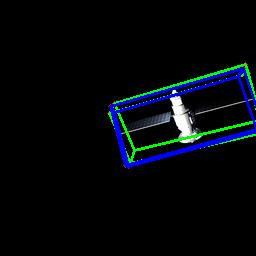
\includegraphics[width=\linewidth]{data/fig9.jpg} % First image
        \caption{Cosmos Link, no background, 256x256 query image, $e_\mathrm{ADD}=1.925$, $e_{\mathrm{ADD}\text{-}\mathrm{S}}=0.377$ }
        \label{fig:fig9}
    \end{minipage}\hfill
    \begin{minipage}{0.45\linewidth}
        \centering
        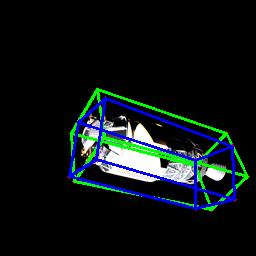
\includegraphics[width=\linewidth]{data/fig10.jpg} % Second image
        \caption{Rocket Body, no background, 256x256 query image, $e_\mathrm{ADD}=1.982$, $e_{\mathrm{ADD}\text{-}\mathrm{S}}=0.501$ }
        \label{fig:fig10}
    \end{minipage}
\end{figure}

\bigskip
\bigskip

From our observations, it's notable that the results are particularly less accurate with the Hubble Space Telescope. This seems to stem from errors in the ground truth poses, as pointed out by Haochen, another student working on the project, particularly an axis inversion. Also, we often notice that the estimations on the Rocket Body are rotated around the object's axis of symmetry compared to the ground truth pose. Thus, it is relevant to consider the $e_{\mathrm{ADD}\text{-}\mathrm{S}}$ metric in this case.

\bigskip

\cleardoublepage{}

While the above results are great, the issue is that in many instances, the estimation is rather inaccurate.
For completeness, we are now studying cases where Gen6D doesn't perform well, and we are trying to identify the reasons behind these shortcomings. The following text is provided by the authors to offer a clearer understanding of the intermediary results presented below: "[The column of vertical images] shows the viewpoint selection results. The first row shows the input image to the selector. The second row shows the input images rotated by the estimated in-plane rotation (left column) or the ground-truth in-plane rotation (right column) Subsequent 5 rows show the predicted (left) or ground-truth (right) 5 reference images with nearest viewpoints to the input image."

\bigskip
\bigskip

\begin{figure}[ht]
  \centering
  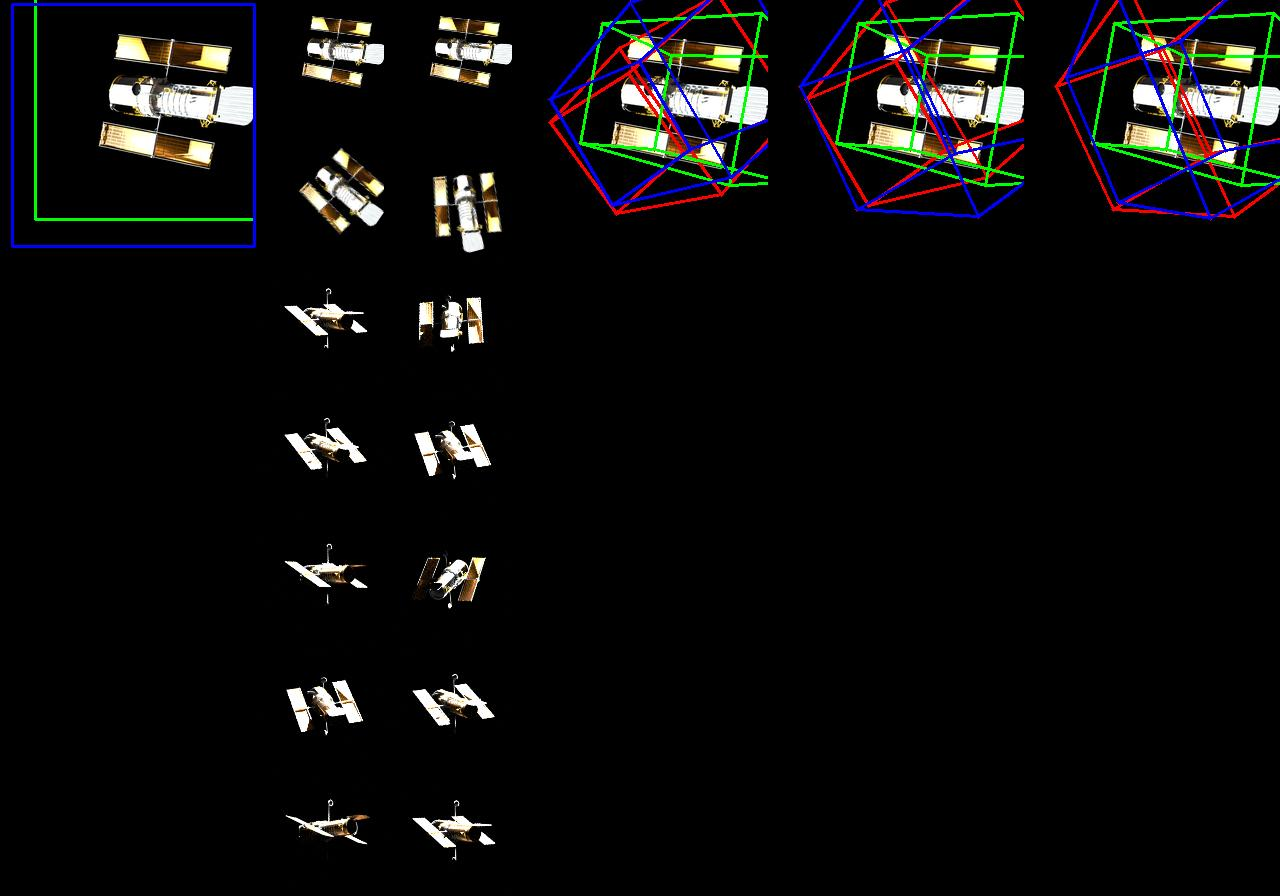
\includegraphics[width=\textwidth]{data/fig11.jpg}
  \caption{Hubble Space Telescope, no background, intermediary result of a poor estimation, $e_\mathrm{ADD}=9.577$, $e_{\mathrm{ADD}\text{-}\mathrm{S}}=5.196$}
  \label{fig:fig11}
\end{figure}

\bigskip

In Figure~\ref{fig:fig11}, we observe good detection of the object, however, the selection of the nearest viewpoint is lacking, ultimately leading to an inaccurate pose estimation. This supports the earlier explanations regarding errors in the ground truth poses for the Hubble Space Telescope. 

\bigskip
\cleardoublepage{}

\begin{figure}[ht]
  \centering
  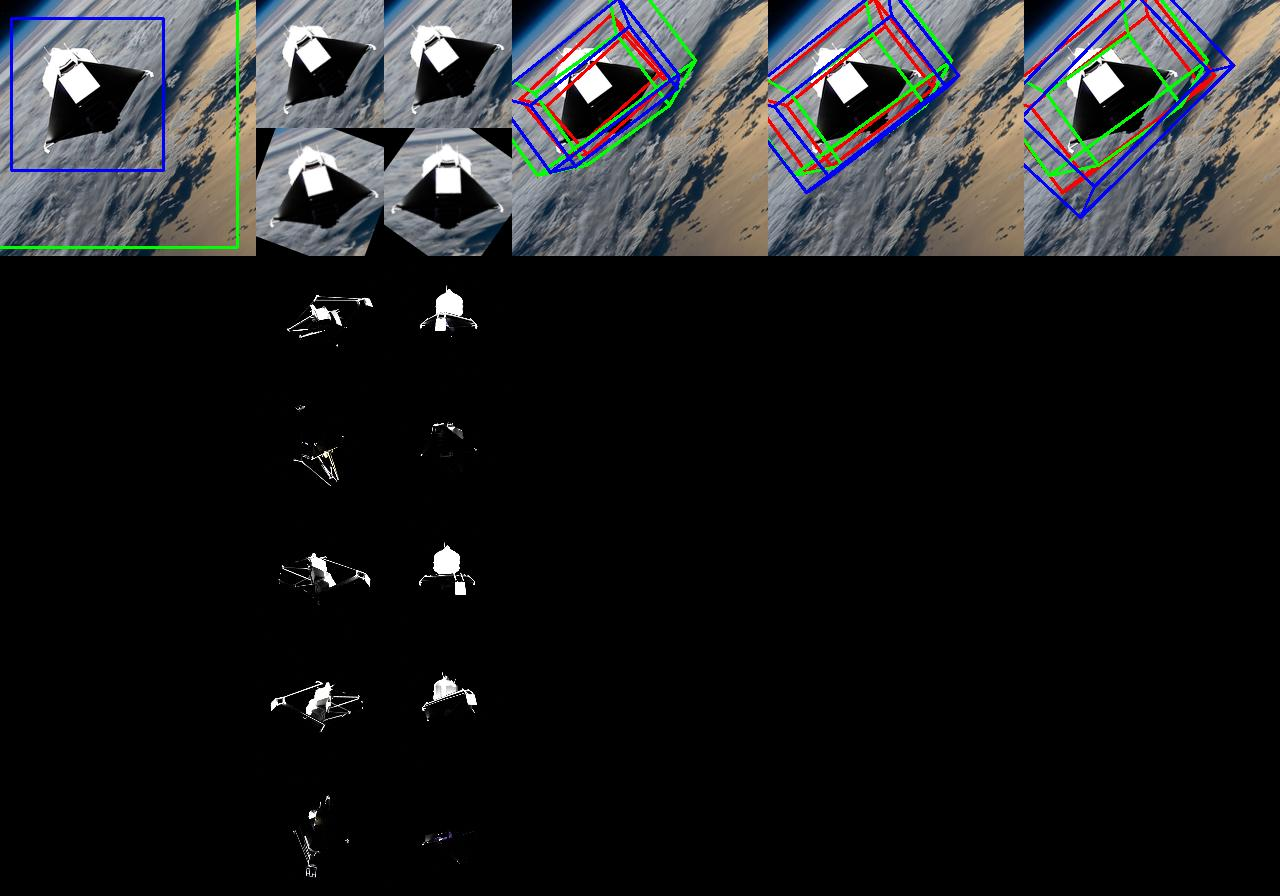
\includegraphics[width=0.8\textwidth]{data/fig12.jpg}
  \caption{James Webb Space Telescope, with earth rendered background, intermediary result of a poor estimation, $e_\mathrm{ADD}=10.934$, $e_{\mathrm{ADD}\text{-}\mathrm{S}}=4.317$}
  \label{fig:fig12}
\end{figure}

\bigskip

\begin{figure}[ht]
  \centering
  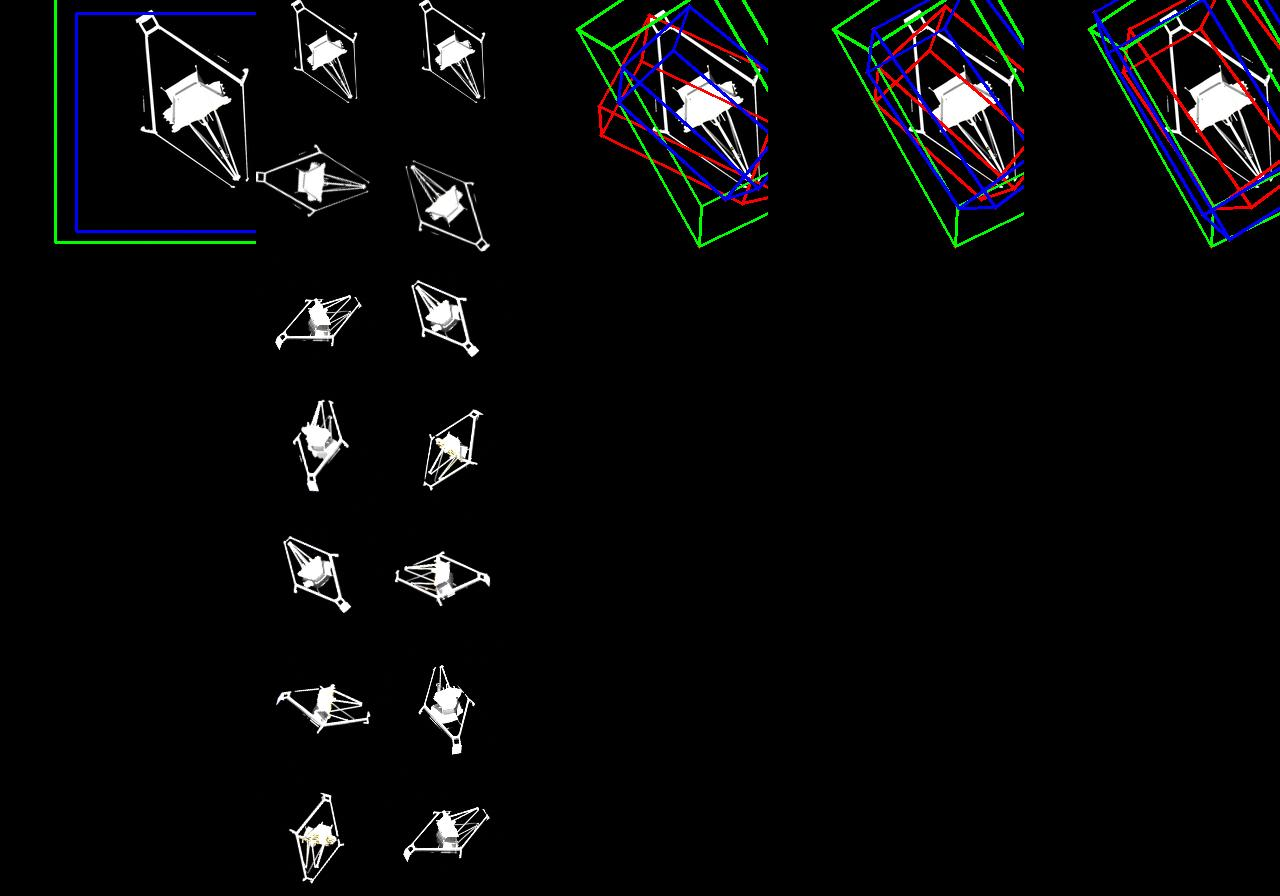
\includegraphics[width=0.8\textwidth]{data/fig16.jpg}
  \caption{James Webb Space Telescope, no background, intermediary result, $e_\mathrm{ADD}=1.060$, $e_{\mathrm{ADD}\text{-}\mathrm{S}}=0.556$}
  \label{fig:fig16}
\end{figure}

\bigskip

In Figure~\ref{fig:fig12}, we tested the model using reference images without a background and query images featuring the James Webb Telescope in front of the blue planet. While the object detection appears reasonably accurate, there is a significant difference in lighting conditions between the reference and query images. On the positive side, the refiner seems to work effectively as we observe an improvement in pose accuracy over the course of the three steps. Figure~\ref{fig:fig16} is another example of the refiner doing great.

\bigskip
\cleardoublepage{}

\begin{figure}[ht]
  \centering
  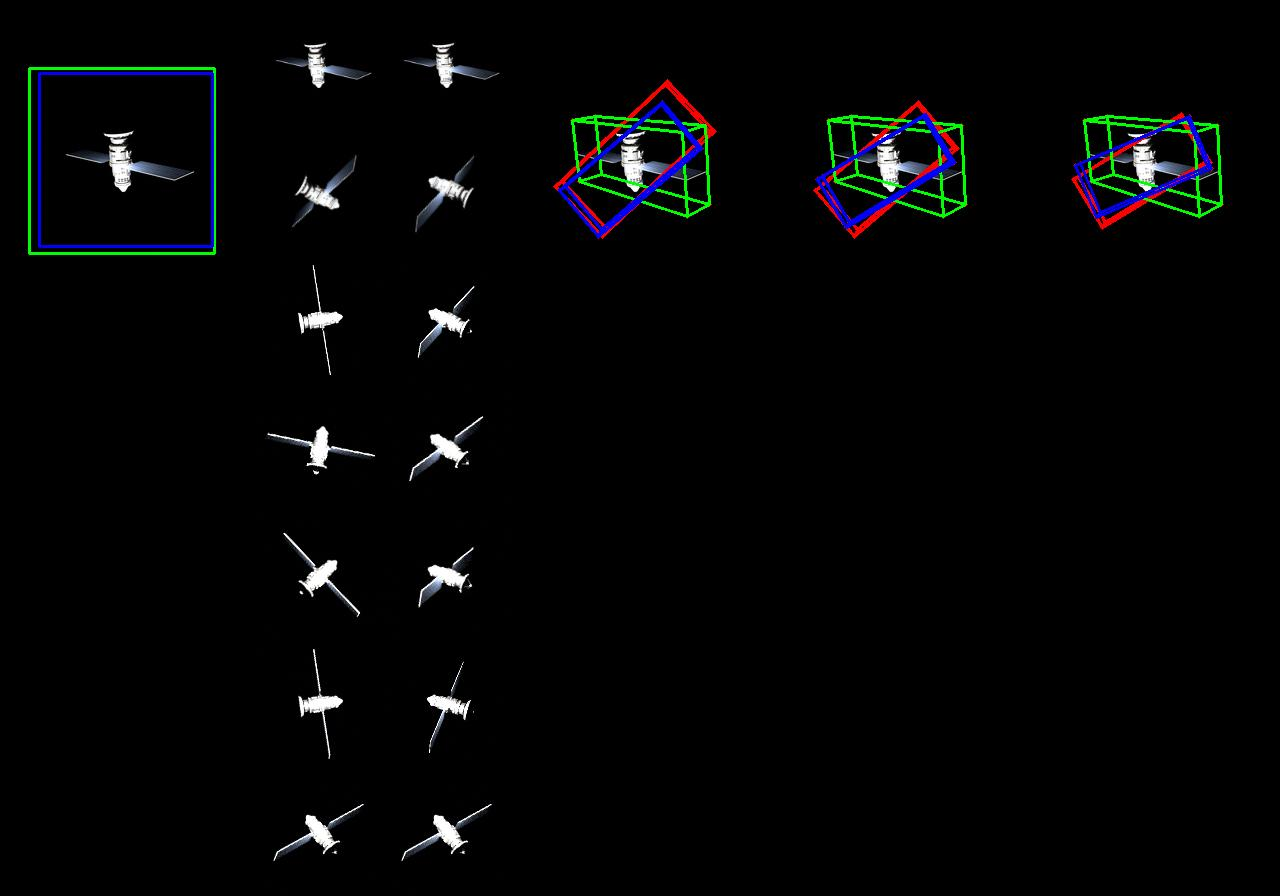
\includegraphics[width=\textwidth]{data/fig13.jpg}
  \caption{Cosmos Link, no background, intermediary result of a poor estimation, $e_\mathrm{ADD}=11.094$, $e_{\mathrm{ADD}\text{-}\mathrm{S}}=6.127$}
  \label{fig:fig13}
\end{figure}

\bigskip

In Figure~\ref{fig:fig13}, we have a perfect detection, reasonably favorable viewpoints and yet a poor estimated pose at the end. However, it appears that increasing the number of refinement steps could lead to an improvement.
\bigskip
\cleardoublepage{}

\begin{figure}[ht]
  \centering
  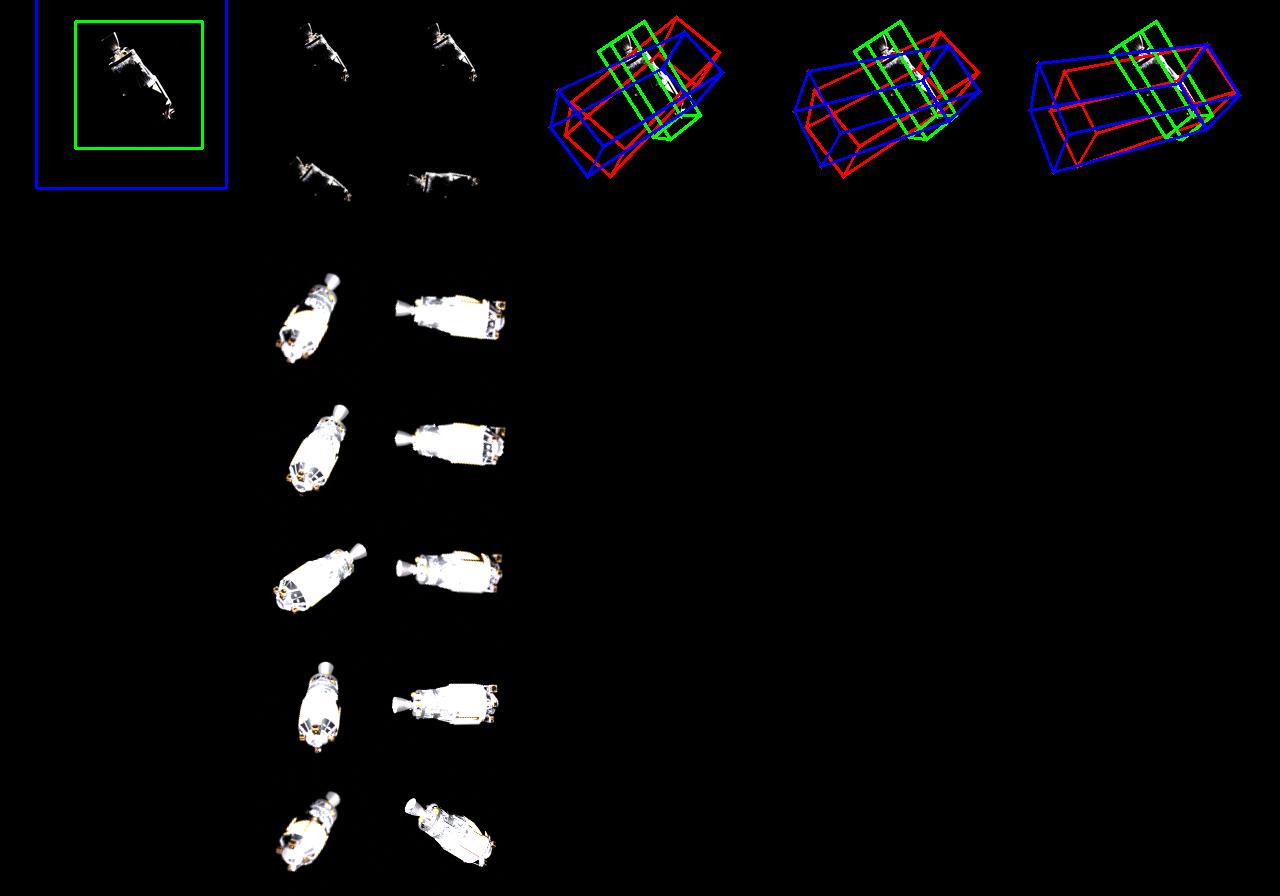
\includegraphics[width=0.8\textwidth]{data/fig14.jpg}
  \caption{Rocket Body, no background, intermediary result of a poor estimation, $e_\mathrm{ADD}=29.335$, $e_{\mathrm{ADD}\text{-}\mathrm{S}}=17.743$}
  \label{fig:fig14}
\end{figure}

\bigskip

\begin{figure}[ht]
  \centering
  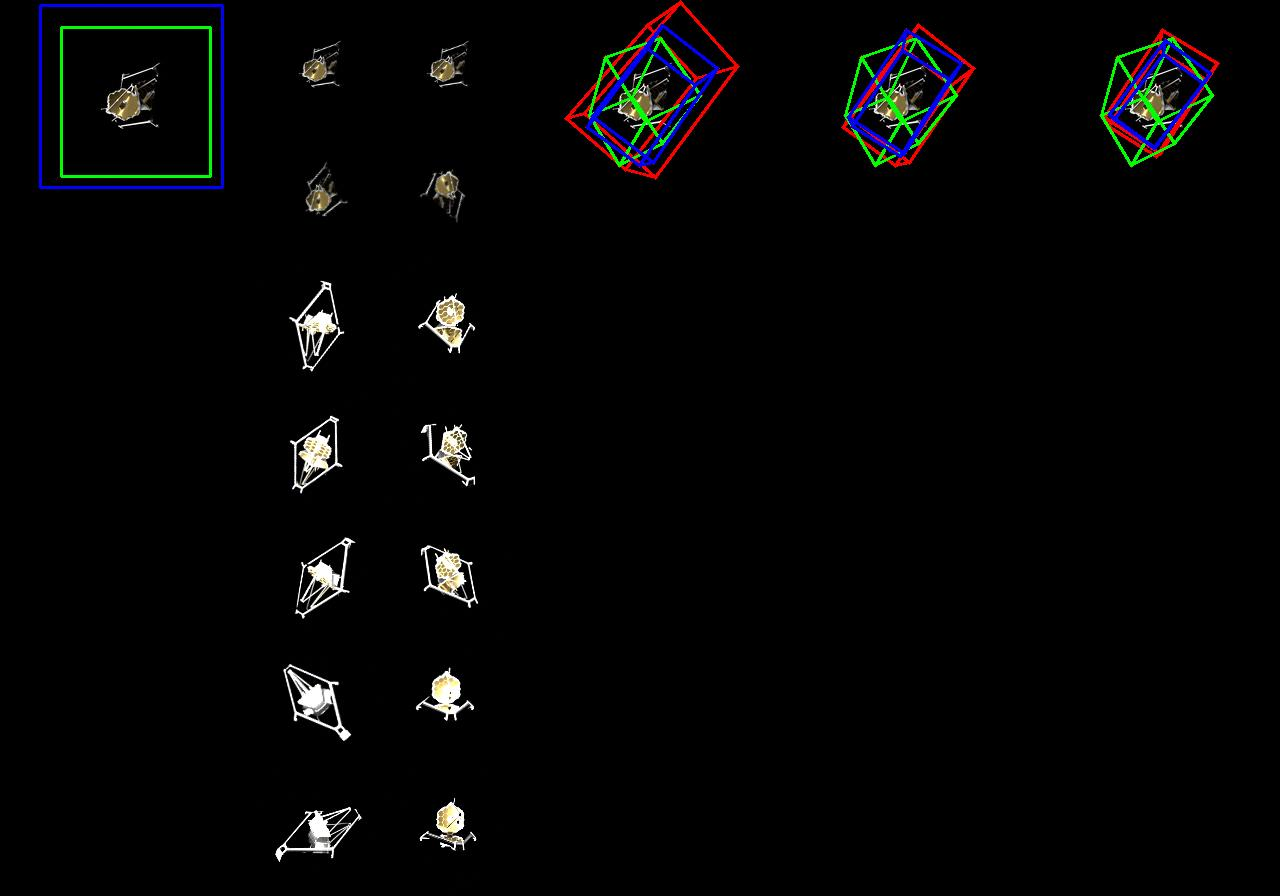
\includegraphics[width=0.8\textwidth]{data/fig15.jpg}
  \caption{James Webb Space Telescope, no background, intermediary result of a poor estimation, $e_\mathrm{ADD}=21.983$, $e_{\mathrm{ADD}\text{-}\mathrm{S}}=12.358$}
  \label{fig:fig15}
\end{figure}

\bigskip

In Figure~\ref{fig:fig14} and Figure~\ref{fig:fig15}, we are encountering large differences in terms of lighting conditions. Specifically, for the James Webb Space Telescope, the query image reveals the interior of the antenna, which is not present in any of the selected viewpoints. Therefore, we conclude that Gen6D struggles with accurately estimating poses when there are substantial variations in lighting conditions.


